\documentclass{BeamerTemplate}
\title{Module 9 - Tests d'hypothèses, partie 1}
\subtitle{STT-1000 Probabilités et statistique}


\usepackage{adjustbox}


\begin{document}
\AtBeginSection{\frame{\sectionpage}}

\begin{frame}

\titlepage

\end{frame}

\section{Introduction}

\begin{frame}[t]{Des hypothèses de recherche}
Une question de recherche est souvent liée à un paramètre d'une population d'intérêt :
\bigskip

\begin{itemize}\itemsep 5mm
%\item la proportion de chômeurs dans une région est inférieure à 6\%;
\item La crue printanière moyenne d'une rivière est supérieure à 8 m.
\item L'écart-type de l'épaisseur des pistons produits par une usine est inférieur à 0,01 cm.
\item Le taux moyen de contaminants diminue après la filtration.
\end{itemize}
\end{frame}

\begin{frame}[t]{Hypothèse statistique}

\begin{Boite}{Hypothèse statistique}{Énoncé sur la loi de probabilité que suit une variable aléatoire (ou sur ses paramètres).}
\end{Boite}

\medskip
Exemples:
\medskip

\begin{tabular}{p{5cm}p{5cm}}
Une population & Plusieurs populations\\
\begin{itemize}
\item $\mu \ne 10$
\item $\mu > 3$
\item $\sigma^2 = 4$
\end{itemize}
&
\begin{itemize}
\item $\mu_1 > \mu_2$
\item $\sigma^2_1 \ne \sigma^2_2$
\item $\mu_1=\mu_2=\mu_3=\mu_4$
\end{itemize}
\end{tabular}
\end{frame}



\begin{frame}[t]{Test d'hypothèses}

\small
Dans un \alerter{test d'hypothèses}, on confronte deux hypothèses.
Par exemple,
$$H_0 : \mu = 10 \qquad \mbox{ contre } \qquad  H_1 : \mu > 10.$$

\medskip
 \alerter{$H_0$ : l'hypothèse nulle}. Considérée comme vraie {\it a priori}, celle qui n'entra\^{\i}ne aucun changement (statu quo).

\medskip
\uncover<2->{
 \alerter{$H_1$ : l'hypothèse alternative}.
Celle que l'on cherche à démontrer avec preuves à l'appui.}

\medskip
\uncover<3->{
On suppose que $H_0$ est vraie jusqu'à ce qu'une \underline{preuve suffisante} que $H_0$ n'est pas vraie ait été amassée. La preuve provient des données qui sont observées (données probantes).}

\end{frame}


\begin{frame}[t]{Remarques}
\begin{itemize}\itemsep4mm
\item $H_0$ et $H_1$ sont toujours incompatibles (les événements des deux hypothèses sont mutuellement exclusifs).
\item Dans notre cours, $H_0$ sera toujours une hypothèse simple ($\mu\alerter{=}10$)
\item $H_1$ peut avoir une forme bilatérale ($\mu\ne 10$)\\ ou unilatérale ($\mu<10$ ou $\mu>10$)
\item C'est l'hypothèse de recherche qui dicte le sens de $H_1$.

\end{itemize}
\end{frame}

\begin{frame}[t]%{Événements mutuellement exclusifs}

\centerline{\LARGE \bf \alert{QUIZ !}}
Vous devez valider qu'une structure de béton a une résistance moyenne supérieure à 80 MPa. Vous prélèverez 10 carottes à analyser.
\bigskip

\begin{enumerate}\itemsep 5mm
\item Quelles sont vos hypothèses statistiques?
\item Vous obtenez une moyenne échantillonnale de\\ $\overline x = 81,6$ MPa. Pouvez-vous conclure que votre hypothèse est vérifiée?
\end{enumerate}

\vspace{1.5cm}

\end{frame}
\begin{frame}[t]{Règle de décision}

Issue d'un test: Rejeter ou non $H_0$.
\bigskip

Une \alerter{règle de décision} est formulée \underline{avant} d'observer les données. Elle  prend la forme d'une \alerter{région critique} qui définit pour quels échantillons $H_0$ sera rejetée.

\bigskip

Par exemple, pour
$$H_0 : \mu = 10 \qquad \mbox{ contre } \qquad  H_1 : \mu > 10.$$

on pourrait choisir de

 $$ \mbox{ rejeter $H_0$ si } \overline{x} > 11.$$

 Comment choisir cette valeur critique?
\end{frame}

\begin{frame}[t]{Deux erreurs possibles à l'issue d'un test d'hypothèses}

{\small
\begin{center}
\begin{tabular}{|c||c|c|}\cline{2-3}
\multicolumn{1}{c||}{ }&\multicolumn{2}{c|}{\bf Réalité (inconnue!)}\\\hline
{\bf Décision} & $  {H_0}$   est vraie  & $ {H_0}$  est fausse \\ \hline\hline
  On rejette $ H_0 $ & \alerter{Erreur de type I} & \\ \hline
  On ne rejette pas  $ H_0 $ & & \alerter{Erreur de type II} \\ \hline
\end{tabular}
\end{center}

\uncover<2->{
%Les règles de décision doivent limiter les chances de commettre des erreurs.
On aimerait contrôler les quantités suivantes:

\vspace{3mm}

$\begin{array}{l|l}
\begin{array}{ll}
\alerter{\alpha}&=P(\text{erreur de type I})\\
&= P(\text{rejeter }H_0 | H_0\text{\ vraie})\\
&= \textbf{\underline{seuil} du test}\\ &\\
\end{array}&
\begin{array}{ll}
\alerter{1-\beta}&=P(\text{rejeter }H_0 | H_0\text{\ fausse})\\
&= P(\text{rejeter }H_0 | H_1\text{ vraie})\\
&= \textbf{\underline{puissance} du test}\\&\\
\end{array}
\\\hline
&
\begin{array}{ll}
\alerter{\beta}&=P(\text{erreur de type II}) \\
&= P(\text{ne pas rejeter }H_0 | H_0\text{\ fausse})\\
\end{array}
\end{array}$
}
}
\end{frame}


\begin{frame}[t]{Quelques remarques}
\begin{itemize}\itemsep4mm
\item {\bf L'erreur de type I  est la plus grave}, donc $\alpha$ est fixé par le chercheur à une faible valeur (souvent $\alpha=0,05$ ou $0,01$).
\item Plus $\alpha$ est petit, plus $\beta$ est grand...\\on contrôlera souvent $\beta$ avec la taille d'échantillon.
\end{itemize}
\end{frame}

\begin{frame}[t]{Exemple 1}

{\small
Une usine affirme qu'elle ne pollue pas le lac avoisinant et que la concentration moyenne de mercure dans le sol au fond du lac ne dépasse pas 0,1 ppm. \\Un biologiste souhaite démontrer le contraire.
}
\medskip

{\small
Il prévoit tirer 10 prélèvements du sol au fond du lac et en mesurer la concentration de mercure. Il suppose que les concentrations sont i.i.d. $N(\mu,\;0,02^2)$. Les hypothèses sont:}

\bigskip
%$H_0:~\mu=0.10$ et $H_1:~\mu>0.10$.
$H_0:$\\[4mm] $H_1:$

\end{frame}
\begin{frame}[t]{Exemple 1 (suite)}

Le biologiste hésite entre deux règles de décision.

\begin{description}
\item[\bf Règle 1:] Rejeter $H_0$ si la concentration moyenne des 10 prélèvements   est supérieure à 0,11.
\item[\bf Règle 2:] Rejeter $H_0$ si la concentration moyenne des 10 prélèvements   est supérieure à 0,12.
    \end{description}

\vspace{7mm}
\begin{itemize}
\item<2->   Comment se comparent les seuils associés à ces deux règles ?
\item<2-> Si la vraie concen\-tration moyenne est $\mu = 0,12$, laquelle des deux règles mène à la plus grande proba\-bilité d'erreur de type II? À la plus grande puissance?
\end{itemize}
\end{frame}

\begin{frame}[t]{Exemple 1: Règle 1, rejet de $H_0$ si $\overline x > 0,11$}
\begin{center}
    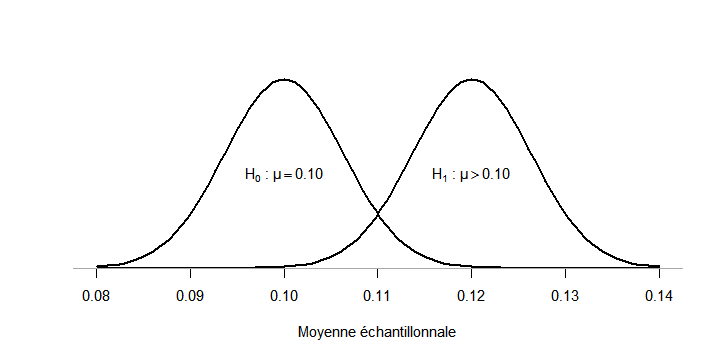
\includegraphics[width=12.5cm]{H0-xbarre.png}
\end{center}

\end{frame}


\begin{frame}[t]{Exemple  1 : Règle 2, rejet de $H_0$ si $\overline x > 0,12$}
\begin{center}
    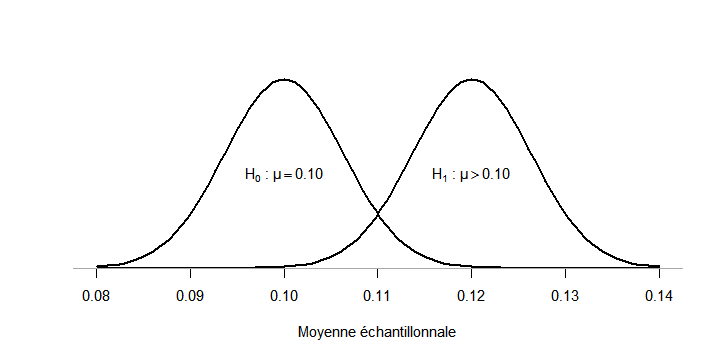
\includegraphics[width=12.5cm]{H0-xbarre.png}
\end{center}
\end{frame}
\begin{frame}[t]{Exemple  1 : Calculs complets}

Vous pourrez vérifier en exercice les valeurs des probabilités d'erreur suivantes:

\begin{center}
{\renewcommand{\arraystretch}{1.5}
\begin{tabular}{|c||c|c|}\cline{2-3}
\multicolumn{1}{c||}{ }&\multicolumn{2}{c|}{\bf Règle de décision}\\\hline
{\bf Probabilité} & Rejeter $H_0$ si $\overline x >0,11$  & Rejeter $H_0$ si $\overline x >0,12$ \\ \hline\hline
$\alpha$   & 0,057 & 0,0008\\ \hline
 $\beta$ (pour $\mu=0,12$)   & 0,057 & 0,5 \\ \hline
 $1-\beta$ (pour $\mu=0,12$)& 0,943 & 0,5 \\ \hline
\end{tabular}
}
\end{center}
{\ }
\end{frame}

\begin{frame}{5 cas étudiés}

La règle de rejet de $H_0$  doit être basée sur la distribution échantillonnale de notre estimateur ($\overline X$ ou $S^2$). Nous considérerons 5 situations pour les tests d'hypothèses à un échantillon (les mêmes que pour les IC):
\vspace{0.3cm}
\small

\begin{tabular}{|c|c|l|}
  \hline
  Cas&Hyp. nulle  & Situation \\\hline
&&\\[-0.3cm]
1&   & $X_1, ..., X_n\;\sim\;N(\mu, \, \sigma^2)$ avec $\sigma^2$ connue \\
&&\\
2& $H_0:\mu=\mu_0$ & $X_1, ..., X_n\;\sim\;N(\mu, \, \sigma^2)$ avec $\sigma^2$ inconnue  \\
&&\\
3&   & $X_1, ..., X_n\;\sim\;$ loi inconnue, mais $n$ est grand  \\[0.2cm]\hline
&&\\[-0.3cm]
4& $H_0:p=p_0$   & $X_1, ..., X_n\sim \text{Bernoulli}(p)$, $n$ assez grand  \\[0.2cm]\hline
&&\\[-0.3cm]
5& $H_0:\sigma^2=\sigma^2_0$& $X_1, ..., X_n\;\sim\;N(\mu, \, \sigma^2)$ \\[0.2cm]\hline
\end{tabular}
\normalsize
\vspace{0.7cm}

\end{frame}

%%%%%%%%%%%%%%%%%%%%%%%%%%%%%%%%%%%%%%%%%%%%%%%%%%%%%%%%%%%%%%%%%%%%%%%%%%%%%%%%%%%%%
\section{Tests d'hypothèses sur la moyenne d'une distribution normale de variance connue}

\begin{frame}[t]{Cas 1: Test sur $\mu$, loi normale, $\sigma^2$  connue}

Supposons un échantillon aléatoire  $X_1,\ldots,X_n$ issu d'une population $N(\mu, \sigma^2)$ où $\mu$ est inconnue mais $\sigma^2$ est connue.

\bigskip
{\bf Objectif:}
Tester si l'échantillon contient suffisamment de "preuves" pour rejeter $H_0:~\mu=\mu_0$, où $\mu_0$ est une valeur donnée.

\bigskip
Trois hypothèses alternatives possibles:

$H_1 : \mu \ne \mu_0$ (bilatérale) \\
$H_1 : \mu < \mu_0$ (unilatérale à gauche) \\
$H_1 : \mu > \mu_0$ (unilatérale à droite) \\
\end{frame}



\begin{frame}[t]{Contre-hypothèse bilatérale}

\small
Tester $H_0 : \mu = \mu_0 \quad\mbox{ contre }\quad \alerter{H_1 : \mu \ne \mu_0}.$

\bigskip

On se doute que \alerter{si $\overline{x}$ s'éloigne trop de $\mu_0$}, c'est que $H_0$  est probablement fausse.

\bigskip

Pour déterminer à partir de quelles valeurs $\overline x$ "s'éloigne trop" de $\mu_0$, on
fixe le seuil $\alpha$ à une petite valeur, comme $0,05$ ou $0,01$.
\bigskip

on cherche $C$ telle que
$$\begin{array}{ll}\alpha &= P(\text{Rejeter } H_0\;|\; H_0 \text{ est vraie})\\&= P\left(\left.|\overline{X}-\mu_0|>C\;\right|\;H_0\mbox{\ est vraie}\right)\end{array}$$

\end{frame}

\begin{frame}[t]{Région critique bilatérale}
\begin{center}
   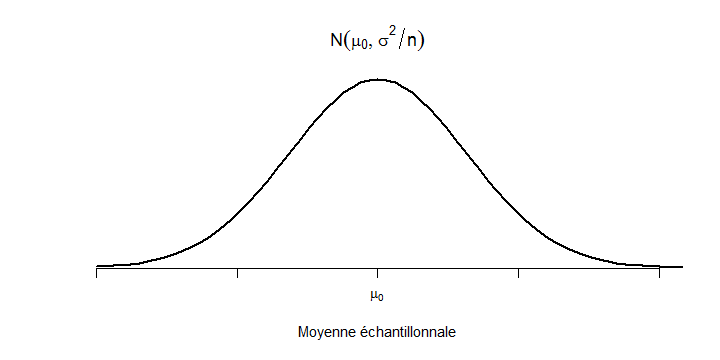
\includegraphics[width=7.5cm]{H0-xbarre-gen.png}

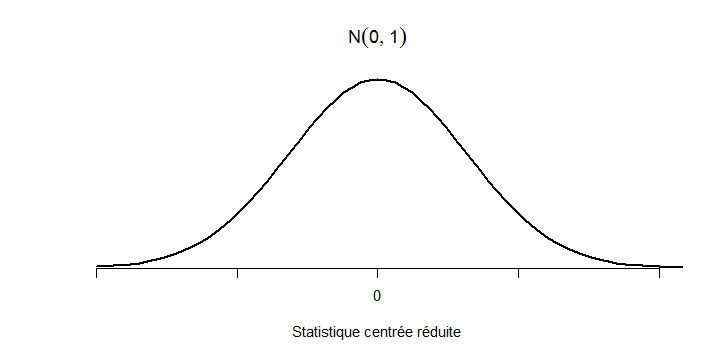
\includegraphics[width=7.5cm]{H0-z.png} 
\end{center}


\end{frame}

\begin{frame}[t]{Région critique bilatérale}
Autrement dit, on rejette $H_0$ au seuil $\alpha$ quand
$$|\overline{X}-\mu_0|>z_{\alpha/2}\sigma/\sqrt{n}.$$

Une fa\c{c}on un peu plus efficace d'écrire cette règle est de définir
$$
Z_0=\frac{\overline{X}-\mu_0}{\sigma/\sqrt{n}}
$$
et de dire que l'on rejette $H_0$ (au profit de $H_1:\mu\ne\mu_0$) quand $|z_0|>z_{\alpha/2}$.
\end{frame}

\subsection{Contre-hypothèses unilatérales}

\begin{frame}[t]{Contre-hypothèses unilatérales}

{\small
\underline{$H_1$ unilatérale à droite:}

Si on veut tester $H_0 : \mu = \mu_0 \mbox{ vs } \alerter{H_1 : \mu > \mu_0}$ alors on rejette $H_0$ si $\overline{x}$ est suffisamment plus élevée que $\mu_0$.

\medskip
Pour obtenir un  test de seuil $\alpha$, on rejette $H_0$ si \alerter{$z_0>z_\alpha$}.

\medskip
\uncover<2->{
\underline{$H_1$ unilatérale à gauche:}

De même, si on veut tester $H_0 : \mu = \mu_0 \mbox{ vs }\alerter{H_1 : \mu < \mu_0}$ alors on rejette $H_0$ pour de faibles valeurs de $\overline{x}$, soit lorsque \alerter{$z_0<-z_\alpha$}.
}
}
\end{frame}


\begin{frame}[t]{Exemple 2}

{\small
Une compagnie affirme que le remboursement d'impôt moyen aux étudiants qui ont utilisé
son service est d'au moins $1100 \,\$$. \\
Un échantillon aléatoire de 20 étudiants ayant utilisé le service ont obtenu un  remboursement moyen de $1060 \,\$$. \\
En supposant une distribution normale d'écart-type $100 \,\$$ pour le remboursement d'un étudiant, peut-on conclure que la compagnie fait de la fausse publicité, au seuil $\alpha = 0,05$ ?}\\

\bigskip

{\bf 1. Hypothèses:}
\bigskip

{\bf 2. Règle de décision:}

\end{frame}

\begin{frame}[t]{Exemple 2 (suite)}

{\bf 3. Calcul de la statistique observée:}

\vfill
{\bf 4. Décision:}

L'hypothèse nulle...

\bigskip
{\bf 5. Conclusion:} (dans les termes de l'étude)

Au seuil de 5\%, le remboursement moyen ...
\bigskip
\end{frame}

\subsection{Seuil observé (valeur P)}

\begin{frame}[t]{Le seuil observé ou valeur-p d'un test ({\it p-value})}

\begin{Boite}{Seuil observé ou valeur-p}
{\small Le seuil observé d'un test,  noté $\alpha^*$,  est la \alert{plus petite valeur de $\alpha$} pour laquelle cet échantillon nous permettrait de rejeter  $H_0$.

 \vspace{3mm}

 $\alpha^*$ peut être vu comme la \alert{probabilité d'observer un autre échantillon  ``au moins aussi extrême'' sous $H_0$.}}
\end{Boite}


\uncover<2->{
\begin{center}
\framebox{On rejette $H_0$ au seuil $\alpha\quad\Leftrightarrow\quad\alpha^*\le\alpha$.}
\end{center}
}
\end{frame}


\begin{frame}[t]{Interprétation du seuil observé}

 $\alpha^*$ peut s'interpréter comme \alerter{une mesure de la compatibilité entre $H_0$ et les observations}, c'est la significativité statistique du test.

\vspace{3mm}
\uncover<2->{Plus la valeur-p est faible, moins notre échantillon semble plausible sous $H_0$.}

\vspace{3mm}
\uncover<3->{\alerter{Attention!} La valeur-p ne donne pas d'information sur la distance entre $\mu_0$ et le "vrai" $\mu$ (ou n'importe quel paramètre d'intérêt).}

\end{frame}

\begin{frame}[t]{Exemple 1 (retour)}

{\small
Retournons à l'exemple sur la concentration de mercure. Si la concentration moyenne observée pour les 10 prélèvements est de 0,111 ppm, quel est le seuil observé du test?}\\

\begin{center}
    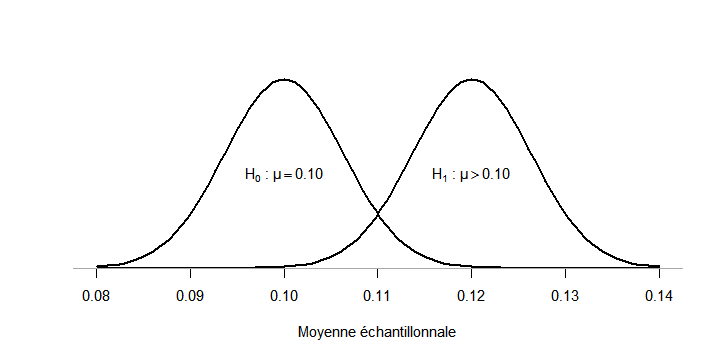
\includegraphics[width=10.5cm]{H0-xbarre.png}
\end{center}

\end{frame}

\begin{frame}[t]{Exemple 1 (suite)}

{\ }
\end{frame}
\begin{frame}[t]%{Événements mutuellement exclusifs}

\centerline{\LARGE \bf \alert{QUIZ !}}
Vous faites un test sur 20 observations  pour confronter les hypothèses $H_0: \mu=5$ et $H_1: \mu<5$. Vous obtenez un seuil observé (valeur P) de 0,09.

Vrai, faux ou manque d'information?
\begin{enumerate} \itemsep 3mm
\item La moyenne échantillonnale est inférieure à 5.
\item Vous rejetez $H_0$ au seuil de 5\%.
\item Vous rejetez $H_0$ au seuil de 10\%.
\item Vous rejetez $H_0: \mu=4$ contre $H_1: \mu<4$ au seuil de 5\%.
\item Vous rejetez $H_0: \mu=6$ contre $H_1: \mu<6$ au seuil de 5\%.
\item Vous refaites l'expérience avec 40 observations. Vous obtenez la même moyenne échantillonnale. Votre seuil observé est alors plus élevé que 0,09 pour le test $H_0: \mu=5$ contre $H_1: \mu<5$.
\end{enumerate}

\end{frame}

\begin{frame}[t]{Formules pour le seuil observé}

 {\small
 De la définition du seuil observé $\alpha^*$, on peut facilement déduire
les formules générales suivantes (pour le cas 1: loi normale, $\sigma^2$ connue):

 \begin{itemize}\itemsep4mm
 \item Pour $H_0 : \mu = \mu_0 \mbox{ vs } H_1 : \mu \neq \mu_0$:\\
 $\alpha^*=P(|Z|>|z_{0}|)=2\,P(Z>|z_{obs}|)$.
 \item Pour $H_0 : \mu = \mu_0 \mbox{ vs } H_1 : \mu > \mu_0$:\\
 $\alpha^*=P(Z>z_{0})$.
 \item Pour $H_0 : \mu = \mu_0 \mbox{ vs } H_1 : \mu < \mu_0$:\\
 $\alpha^*=P(Z<z_{0})$.
 \end{itemize}
 }
\end{frame}

\begin{frame}[t]{Exemple 2 (suite)}
Quel est le seuil observé du test réalisé sur la moyenne des remboursements d'impôts?
{\ }
\end{frame}



\subsection{Puissance et taille d'échantillon}

\begin{frame}[t]{Calcul de puissance}

\begin{itemize}\itemsep7mm
\item Rappel: $$\text{Puissance du test}=P(\text{ rejeter } H_0\,|\,H_1 \text{  est vraie}).$$
\item En général, $H_1$ ne spécifie pas une valeur unique de $\mu$, mais un intervalle de valeurs.
\item On calcule la puissance pour une valeur plausible ou arbitraire de $\mu$ sous $H_1$, que nous noterons $\mu_1$.
\end{itemize}
\end{frame}

\begin{frame}[t]{Exemple 3}
On pige un échantillon $X_1, \ldots, X_{16}$  d'une loi $N(\mu, 64)$ pour tester, au seuil $\alpha = 0,10$:

 $$\begin{array}{ll}
 H_0 : &\mu = 10\\ H_1 : &\mu > 10
 \end{array}$$

 Quelle est la puissance du test si en vérité $\mu = 11$?
\end{frame}

\begin{frame}[t]{Exemple 3 (suite)}

{\ }

\end{frame}

\begin{frame}[t]{Déterminants de la puissance}

{\small
Trois facteurs importants influencent la puissance d'un test:}

\begin{enumerate}
\item[1.] \alerter{la différence entre $\mu_0$ et $\mu_1$}:
plus $\mu_1$ s'éloigne de $\mu_0$, plus la puissance augmente.

\begin{center}
    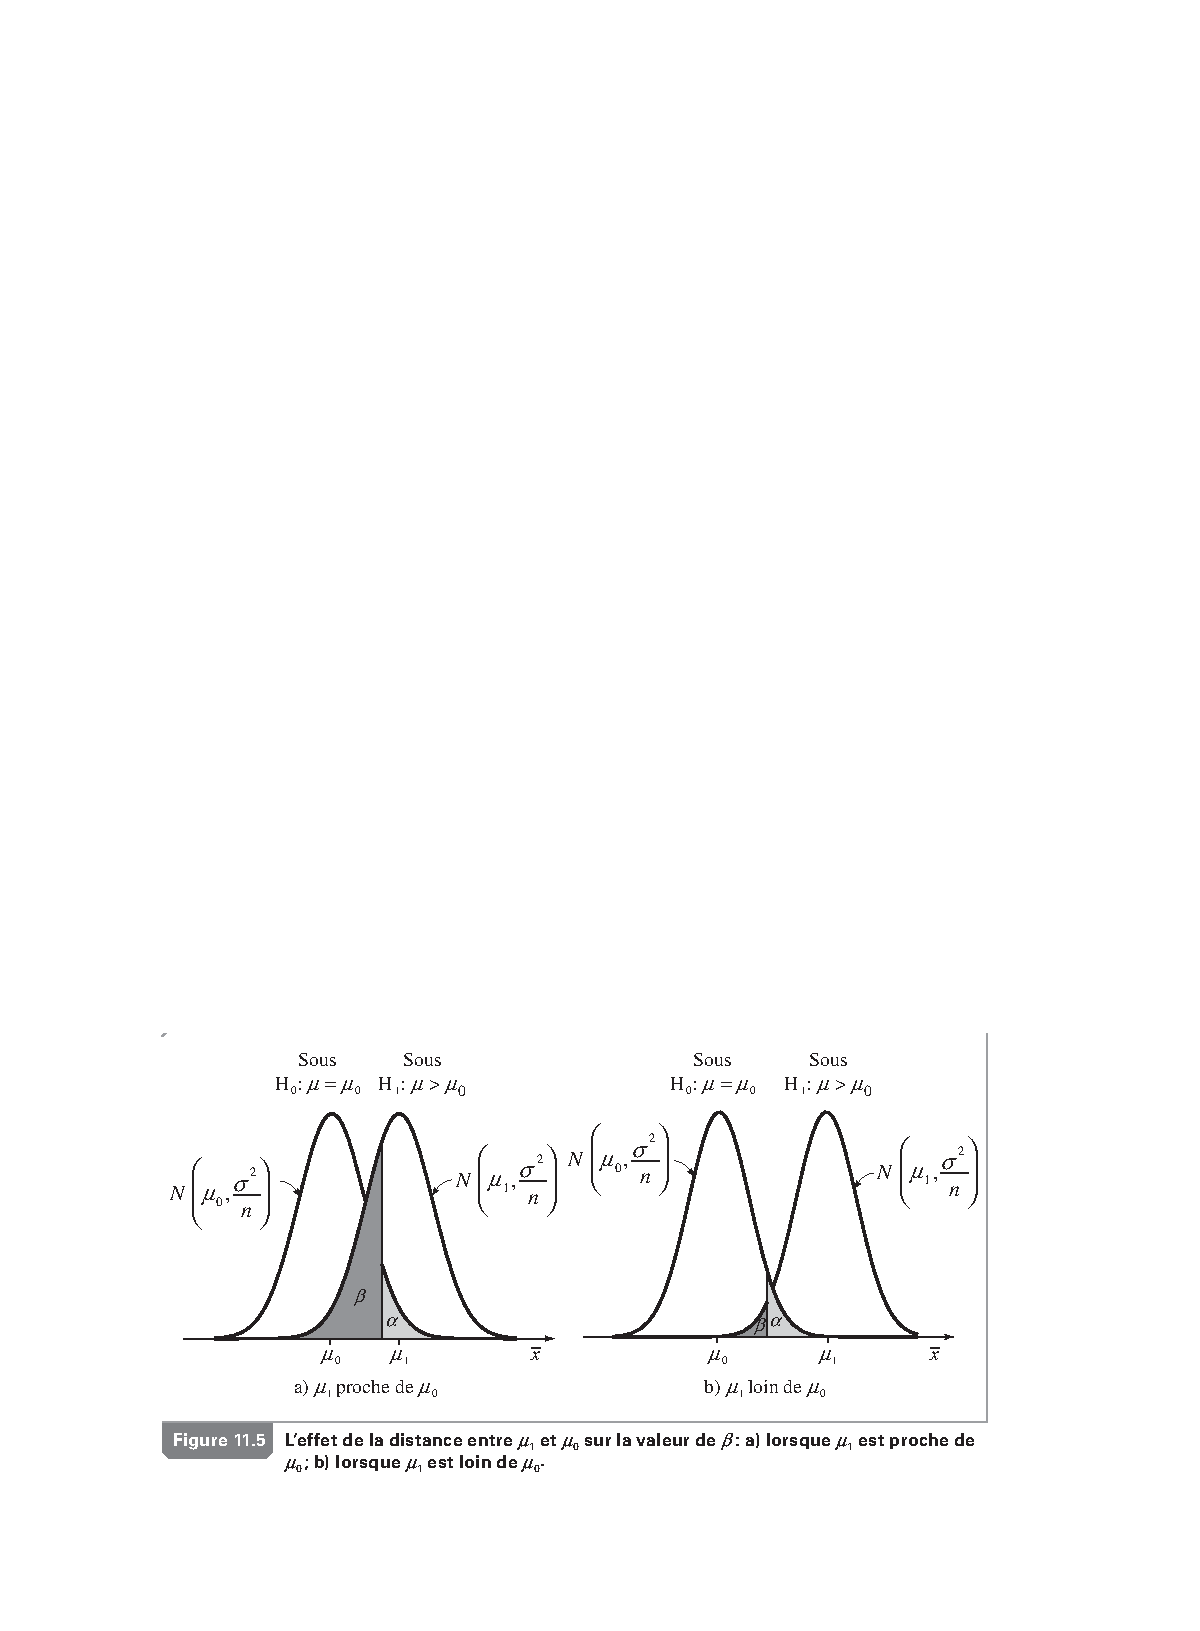
\includegraphics[width=10cm]{puiss1.pdf}

\end{center}

\end{enumerate}
\end{frame}

\begin{frame}[t]{Déterminants de la puissance}

\begin{enumerate}
\item[2.] \alerter{le seuil du test}:
plus $\alpha$ augmente, plus la puissance augmente;

\begin{center}
    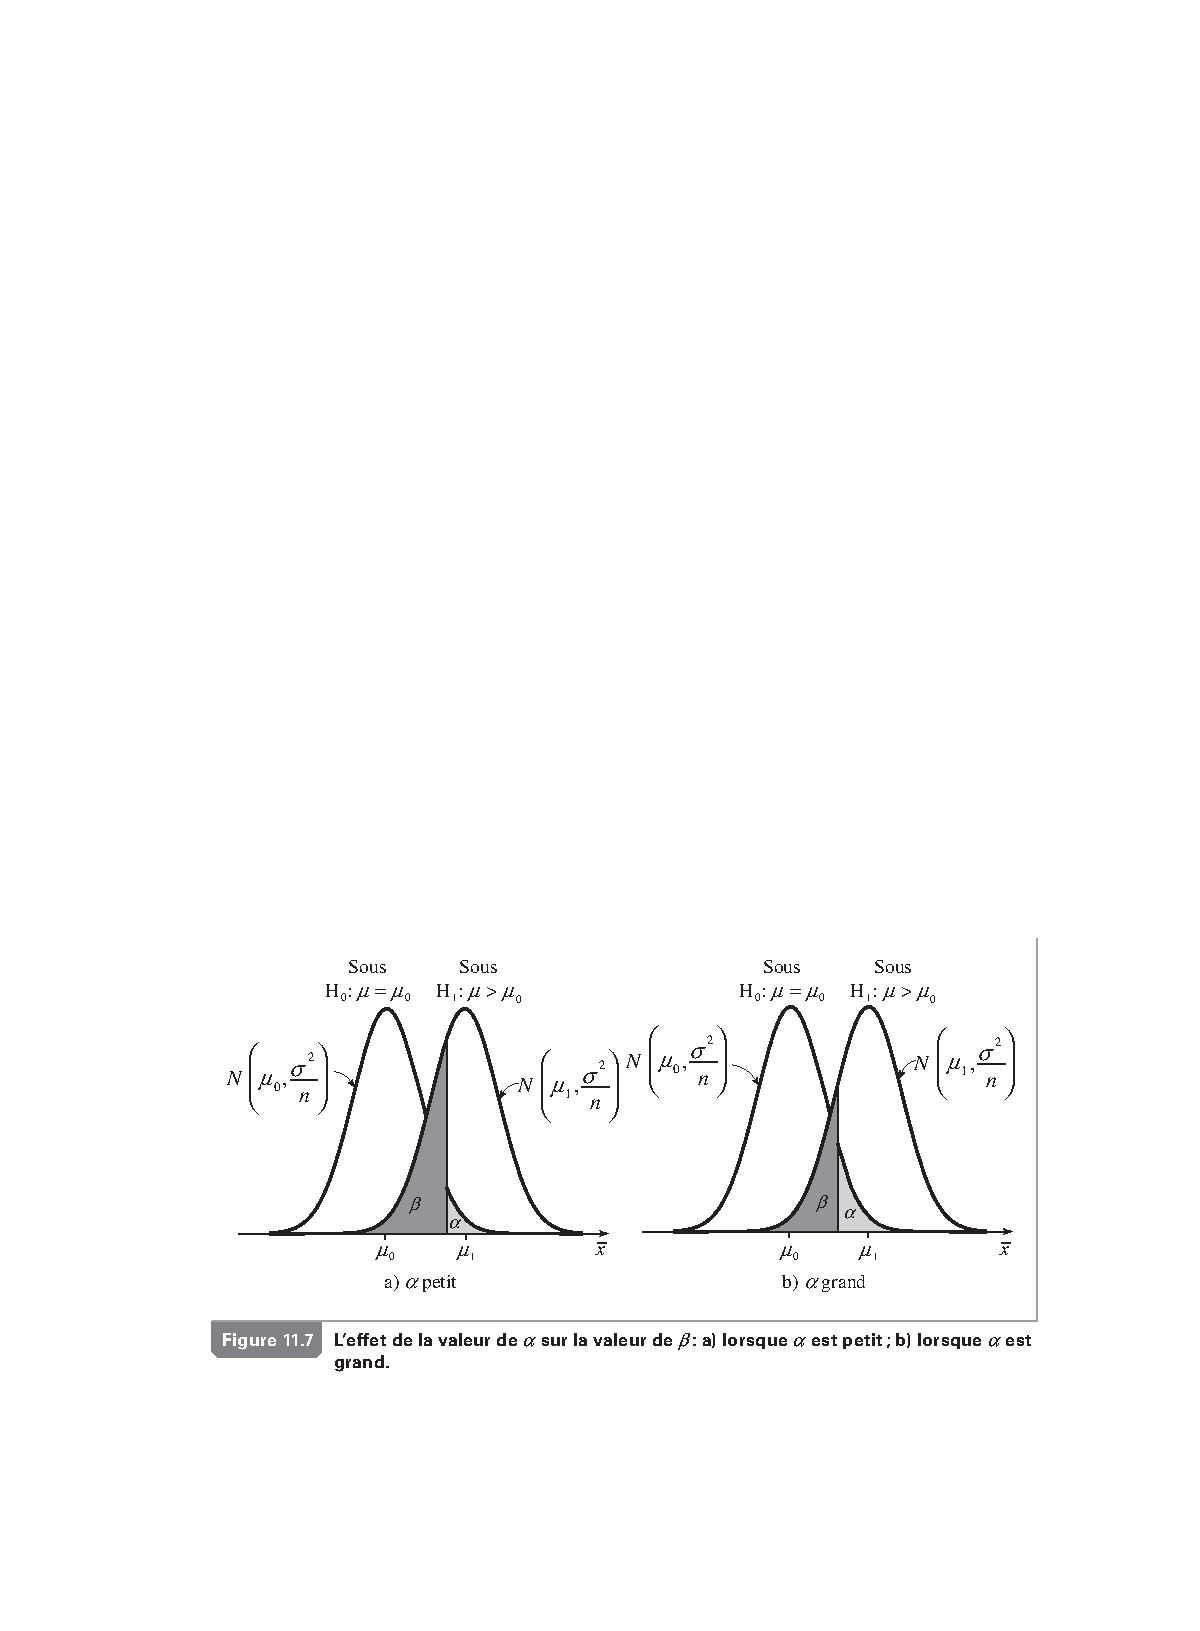
\includegraphics[width=10cm]{puiss3.pdf}

\end{center}
\end{enumerate}
\end{frame}


\begin{frame}[t]{Déterminants de la puissance}


\begin{enumerate}
\item[3.] \alerter{la taille d'échantillon}: plus $n$ augmente, plus la puissance augmente.

\begin{center}
    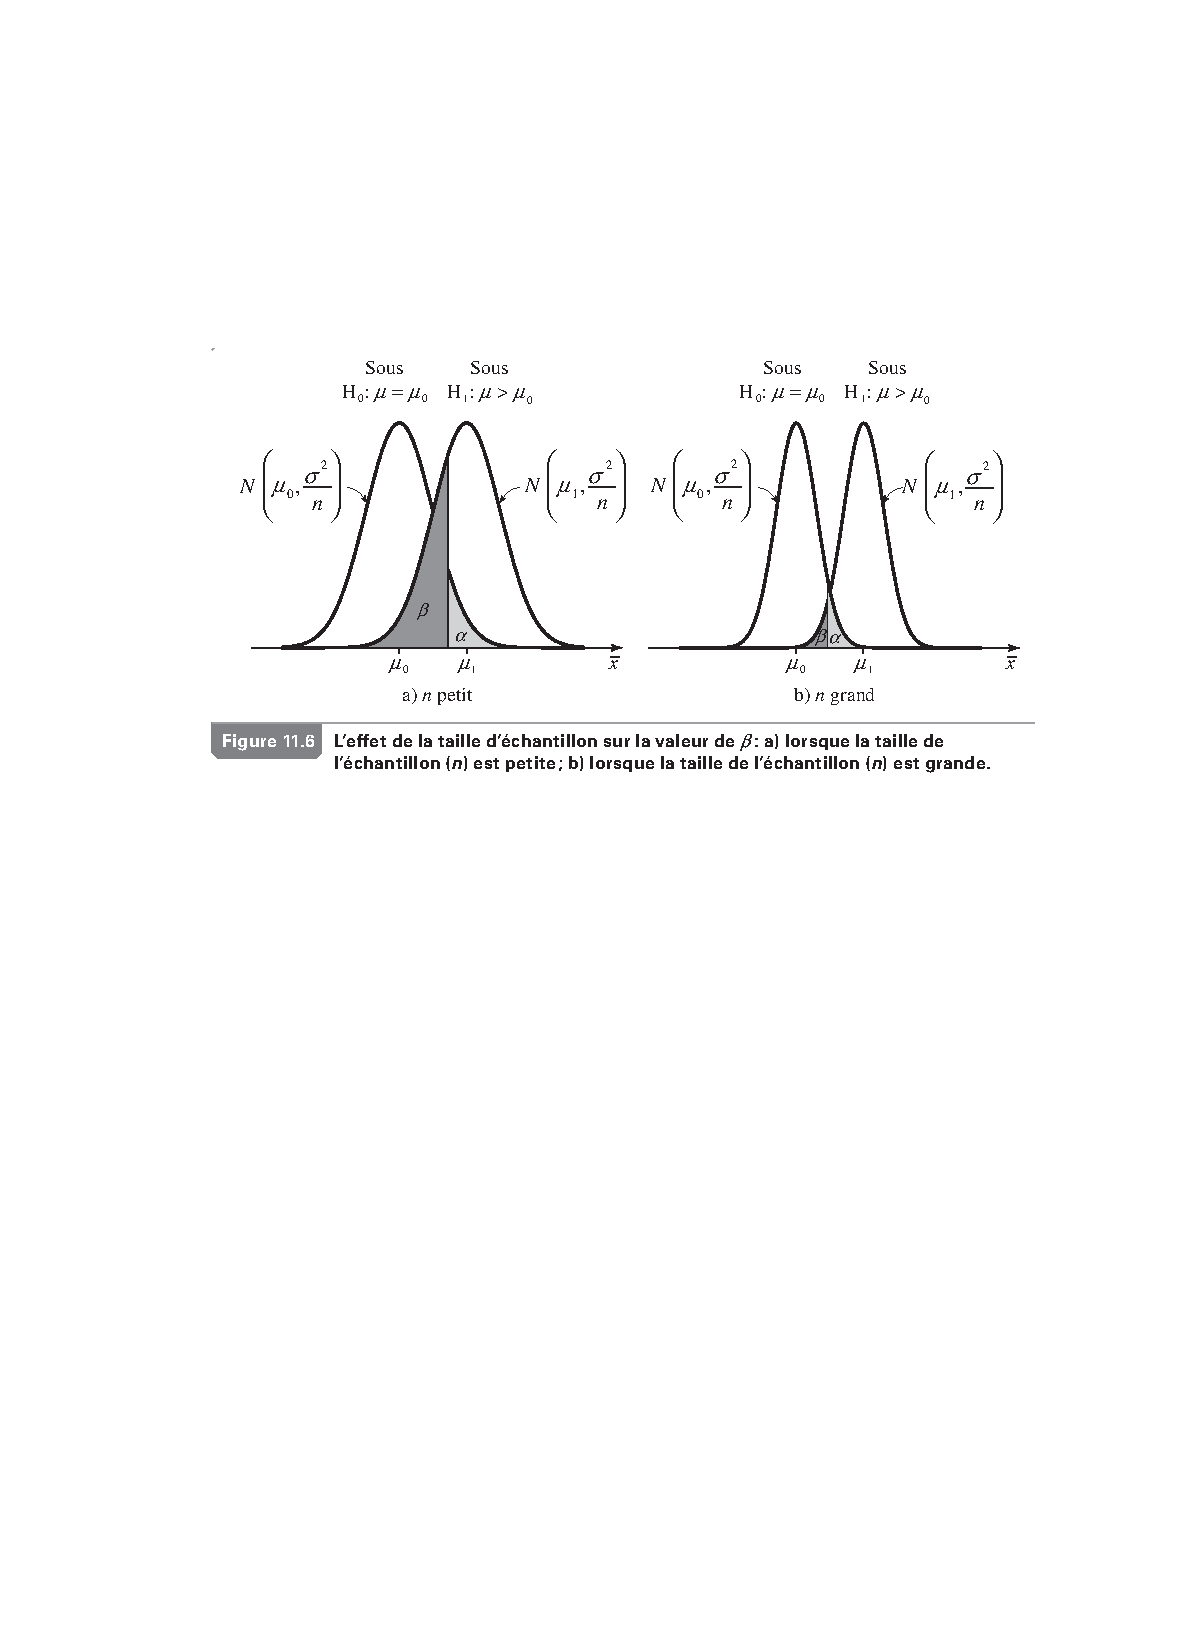
\includegraphics[width=10cm]{puiss2.pdf}

\end{center}

\end{enumerate}
\end{frame}
\begin{frame}[t]{Déterminants de la puissance}

\begin{enumerate}\itemsep5mm
\item Le statisticien n'a aucun contrôle sur $\mu$, la vraie valeur de la moyenne. Il peut demander au chercheur la plus petite différence qu'il considère importante.

\item On peut augmenter $\alpha$ pour augmenter la puissance, mais on augmente les chances de faire une erreur de type I.

\item En pratique, \alerter{la seule option est souvent d'augmenter la puissance en choisissant $n$ suffisamment grand}.
\end{enumerate}
\end{frame}

\begin{frame}[t]{Exemple 3 (retour)}

On reconsidère notre échantillonnage dans une population  $N(\mu, 64)$ pour tester (avec $\alpha = 0,10$)

 $$\begin{array}{ll}
 H_0 : &\mu = 10\\ H_1 : &\mu > 10
 \end{array}$$

Quelle est la taille d'échantillon nécessaire pour que la puissance soit de 80\% si $\mu = 11$?

\end{frame}



%%%%%%%%%%%%%%%%%%%%%%%%%%%%%%%%%%%%%%%%%%%%%%%%%%%%%%%%%%%%%%%%%%%%%%%%%%%%%%%%%%%%%
\section{Tests d'hypothèses sur la moyenne d'une distribution normale de variance inconnue}
\subsection*{ }


\begin{frame}[t]{Cas 2: Tests sur $\mu$,  loi normale, $\sigma^2$ inconnue}

Comment faire un test sur $\mu$ si la variance est inconnue?

\medskip
Le test basé sur $Z_0$ est inapproprié puisque l'erreur de type I qui serait commise
serait  supérieure à $\alpha$.

\medskip

Si la variance est inconnue, on utilise la statistique
$$
T_0 = \frac{\overline{X}-\mu_0}{S/\sqrt{n}}.
$$
Sous $H_0$, on sait que $T_0\sim t_{n-1}$.

\end{frame}

\begin{frame}[t]{Règles de décision}

{\small
Au seuil $\alpha$, on rejette $H_0:\mu=\mu_0$ ...
\begin{itemize}
\item \underline{Test bilatéral ($H_1 : \mu \ne \mu_0$)}:

    \begin{enumerate}[$\circ$]\itemsep2mm
    \item on rejette $H_0$ si $|t_0| > t_{\alpha/2, n-1}$
    \item $\alpha^*=P(|t_{n-1}|>|t_0|)=2\,P(t_{n-1}>|t_0|)$
    \end{enumerate}

\item \underline{Test unilatéral à droite ($H_1 : \mu > \mu_0$)}:

    \begin{enumerate}[$\circ$]\itemsep2mm
    \item on rejette $H_0 : \mu = \mu_0$  si $t_0 > t_{\alpha, n-1}$
    \item $\alpha^*=P(t_{n-1}>t_0)$
    \end{enumerate}

\item \underline{Test unilatéral à gauche ($H_1 : \mu < \mu_0$)}:

    \begin{enumerate}[$\circ$]\itemsep2mm
    \item on rejette $H_0 : \mu = \mu_0$ si $t_0 < -t_{\alpha, n-1}$.
    \item $\alpha^*=P(t_{n-1}<t_0)$
    \end{enumerate}
\end{itemize}
}
\end{frame}

%\subsection{Seuil observé}

\begin{frame}[t]{Seuils observés et puissance}

\underline{Seuils observés}:

Dans tous les cas, on peut énoncer la règle suivante:

\centerline{\alerter{On rejette $H_0$ si $\alpha^*<\alpha$.}}

C'est le calcul de la valeur-P ($\alpha^*$) qui change selon le test.

\bigskip
\uncover<2->{
\underline{Puissance}:

Les calculs de puissance pour le cas 2 font appel à une loi $t$ {\it décentrée} et ne seront donc \alerter{pas couverts dans ce cours}.}
\end{frame}

\begin{frame}[t]{Exemple 4}

Une fabrique achète régulièrement des transistors à un fournisseur. Les données passées montrent que le coefficient d'amplification de ces transistors avait une distribution normale de moyenne 155.

\medskip

Lors d'un nouveau contrôle sur 20 transistors, on observe un coefficient d'amplification moyen de 152 et un écart-type de 10. Peut-on admettre, au seuil de 1\%, que le coefficient  moyen a changé?


\bigskip

{\bf 1. Hypothèses:}
\bigskip

{\bf 2. Règle de décision:}

\end{frame}

\begin{frame}[t]{Exemple 4 (suite)}

{\bf 3. Calcul de la statistique observée:}

\vfill
{\bf 4. Décision:}

L'hypothèse nulle...

\bigskip
{\bf 5. Conclusion:} (dans les termes de l'étude)

Au seuil de 1\%, le coefficient d'amplification moyen ...
\bigskip

\end{frame}


\section{Tests d'hypothèses sur la moyenne d'une loi inconnue}

\begin{frame}[t]{Cas 3: Tests sur $\mu$,  loi inconnue, $n$ grand}

Si la loi théorique des observations en cause est inconnue, comment faire un test sur la moyenne?

\vspace{5mm}

Si $n$ est grand (au moins 30), le test présenté au cas 1 peut être utilisé en rempla\c{c}ant $\sigma$ par l'écart-type échantillonnal $S$ dans la définition de $Z_0$.

\vspace{5mm}

Les probabilités d'erreur de type I et II ($\alpha$ et $\beta$) seront alors approximatives (car la loi normale est un modèle approximatif pour $\overline X$ lorsque $n$ est grand).

\end{frame}

\section{Tests d'hypothèses sur une proportion}

\begin{frame}[t]{Cas 4: Tests sur $p$, loi de Bernoulli}

On suppose que $X_1,\hdots,X_n$ i.i.d. loi Bernoulli$(p)$,
où $p$ inconnue et où $n\geq 30$. \\

Les hypothèses du test bilatéral seront:
 $$\begin{array}{ll}
 H_0 : &p = p_0\\ H_1 : &p \neq p_0
 \end{array}$$
Par le TCL, nous savons que sous $H_0$, $\hat{p}\approx \mathcal{N}(p_0, \frac{p_0(1-p_0)}{n})$ et donc $$Z_0=\frac{\hat{p}-p_0}{\sqrt{\frac{p_0(1-p_0)}{n}}}\approx \mathcal{N}(0,1)$$


 et nous rejetons $H_0$ si $|z_0|>z_{\alpha/2}$.

 Les tests unilatéraux se construisent de façon similaire.
\end{frame}
\section{Tests d'hypothèses sur la variance}
\begin{frame}[t]{Cas 5: Tests sur $\sigma^2$, distribution normale}
Si on veut contrôler la variabilité d'un procédé,
on peut effectuer un test d'hypothèses portant sur la variance d'une distribution.

\medskip
Ces tests sont relativement simples dans le cas où nous
recueillons un \alerter{échantillon aléatoire $X_1,\ldots,X_n$ issu d'une population
$N(\mu,\sigma^2)$}.
\end{frame}

\begin{frame}[t]{Test bilatéral}

%{\small
On suppose $X_1, \ldots, X_n$ un échantillon aléatoire d'une distribution $N(\mu, \sigma^2)$
pour laquelle on veut tester $$\alerter{H_0 : \sigma^2 = \sigma_0^2} \mbox{ contre } \alerter{H_1 : \sigma^2 \ne \sigma_0^2}.$$
On voudra rejeter $H_0$ lorsque $S^2$ sera éloignée de $\sigma^2_0$, donc pour des valeurs éloignées de $n-1$ pour la statistique
$$U_0 = \frac{(n-1)S^2}{\sigma_0^2}. $$

\uncover<2->{
Si $H_0$ est vraie, alors $U_0\sim\chi^2_{n-1}$.\\
Test de seuil $\alpha$:\\
\centerline{\alerter{on rejette $H_0$ si
$u_0<\chi^2_{1-\alpha/2;n-1}$ ou si $u_0>\chi^2_{\alpha/2;n-1}$}.}
}
%}
\end{frame}

\begin{frame}[t]{Tests unilatéraux}

{\small
Au seuil $\alpha$, on rejette $H_0:\sigma^2 = \sigma_0^2$ ...
\begin{itemize}

\item \underline{Test unilatéral à droite ($H_1 : \sigma^2 > \sigma_0^2$)}:

    \begin{enumerate}[$\circ$]\itemsep2mm
    \item on rejette $H_0 : \sigma^2 = \sigma_0^2$  si $u_0>\chi^2_{\alpha;n-1}$
    \item $\alpha^*=P(\chi^2_{n-1}>u_0)$
    \end{enumerate}

\item \underline{Test unilatéral à gauche ($H_1 : \sigma^2 < \sigma_0^2$)}:

    \begin{enumerate}[$\circ$]\itemsep2mm
    \item on rejette $H_0 : \sigma^2 = \sigma_0^2$ si $u_0<\chi^2_{1-\alpha;n-1}$.
    \item $\alpha^*=P(\chi^2_{n-1}<u_0)$
    \end{enumerate}
\end{itemize}
}
\end{frame}


\begin{frame}[t]{Exemple 5}


On évalue une nouvelle machine pour remplir des sacs de sucre. La compagnie est prête à tolérer une variance de 7 g$^2$. Un test sur 31 sacs donne une variance échantillonnale de \mbox{8,2 g$^2$.} La variance est-elle trop grande au seuil \mbox{$\alpha = 0,05$?}


\bigskip

{\bf 1. Hypothèses:}
\vspace{1.5cm}

{\bf 2. Règle de décision:}

\end{frame}

\begin{frame}[t]{Exemple 5 (suite)}

{\bf 3. Calcul de la statistique observée:}

\vfill
{\bf 4. Décision:}

L'hypothèse nulle...

\bigskip
{\bf 5. Conclusion:} (dans les termes de l'étude)

Au seuil de 5\%, la variance des poids ...
\bigskip
\end{frame}


%%%%%%%%%%%%%%%%%%%%%%%%%%%%%%%%%%%%%%%%%%%%%%%%%%%%%%%%%%%%%%%%%%%%%%%%%%%%%%%%%%%%%
\section[Lien IC]{Lien entre intervalles de confiance et tests d'hypothèses bilatéraux}
\subsection*{ }

\begin{frame}[t]{Intervalles de confiance et tests bilatéraux}
Il existe une forte relation entre les intervalles de confiance et les  tests  bilatéraux.

\bigskip
L'examen des régions critiques des tests pour
 $H_0:~\mu=\mu_0$ vs $H_1:~\mu\neq\mu_0$ montre que
 \bigskip

 \begin{tabular}{c c l}
 \alerter{On rejette $H_0:~\mu=\mu_0$ }&  &
 \alerter{L'intervalle de confiance pour $\mu$ }\\
 \alerter{au seuil $\alpha$}& $\Leftrightarrow$ &\alerter{de niveau $1-\alpha$ }\\
 &&\alerter{ne
 contient pas la valeur $\mu_0$}.
 \end{tabular}

 \vspace{1.8cm}

 Idem pour $\sigma^2$.
\end{frame}
\begin{frame}[t]%{Événements mutuellement exclusifs}

\centerline{\LARGE \bf \alert{QUIZ !}}
À la suite d'une étude, on a calculé un intervalle de confiance à 99\% pour $\mu$: $[2,26;\,3,41]$.

\bigskip
Vrai, faux ou manque d'information?

\begin{enumerate}\itemsep 5mm
\item Au seuil de 1\%, on rejette $H_0:\mu=3$ pour $H_1:\mu\ne3$.
\item Au seuil de 1\%, on rejette $H_0:\mu=4$ pour $H_1:\mu\ne4$.
\item Au seuil de 5\%, on rejette $H_0:\mu=3$ pour $H_1:\mu\ne3$.
\item Au seuil de 5\%, on rejette $H_0:\mu=4$ pour $H_1:\mu\ne4$.
\end{enumerate}

\vspace{.5cm}

\end{frame}

\begin{frame}{Bibliographie}
 	Ce document est rédigé avec Beamer ainsi qu'une classe .cls fourni par Jérôme Soucy. Les diapositives sont adaptées des diapositives créées par Thierry Duchesne et Emmanuelle Reny-Nolin pour le cours STT-1900. Les graphiques proviennent de ces mêmes diapositives.
 	\printbibliography
 	\vfill
 	\footnotesize Pour signaler une erreur dans ce document, veuillez écrire à l'adresse :~\href{mailto:julien.miron@mat.ulaval.ca}{julien.miron@mat.ulaval.ca}.
 \end{frame}

\end{document}

